\section{Evaluation}
\label{sec:evaluation}

We evaluate CudeleFS on a 15 node cluster, partitioned into 8 object storage
servers, 3 metadata servers, and 2 monitor servers. The object storage servers
double as clients which is fine because clients are CPU and memory bound while
object storage servers are disk IO bound. All daemons run as a single process
which is the default setting for Ceph and the nodes have 2 dual core 2GHz
processors with 8GB of RAM. There are three daemons per object storage server
(one for each disk formatted with XFS) and they share an SSD for the journal.
The nodes are running Ubuntu 12.04.4, kernel version 3.2.0-63 but all
experiments run in Docker containers; this makes it easier to tear down and
re-initialize the cluster ({\it e.g.}, dropping the kernel cache) between
experiments.

This paper adheres to The Popper
Convention\footnote{\url{http://falsifiable.us}}~\cite{jimenez_popper_2016}, so
experiments presented here are available in the repository for this
article\footnote{Links have been removed for double-blind submission}.
Experiments can be examined in more detail, or even re-run, by visiting the
\texttt{[source]} link next to each figure. That link points to a Jupyter
notebook that shows the analysis and source code for that graph, which points
to an experiment and its artifacts.

%\begin{figure*}[tb]
%\centering
%\includegraphics[width=180mm]{graphs/slowdown.png}
%\caption{Compared to the \texttt{create} phase, saving and persisting
%updates (\texttt{create+save} and \texttt{create+save+persist}) experience only
%a 4.79\(\times\) and 8.66\(\times\) slowdown, in the worst case for 100K files.
%In contrast, maintaining \texttt{global} consistency is 905.70\(\times\)
%slower.  The disadvantage of decoupling the namespace is the merge phase where
%updates are applied to the metadata store (\texttt{create+apply}, resulting in a
%905.70\(\times\) slowdown for 100K files.}\label{fig:global-v-decoupled}
%\end{figure*}

\subsection{CudeleFS Mechanism Performance}

\begin{figure}[tb]
\centering
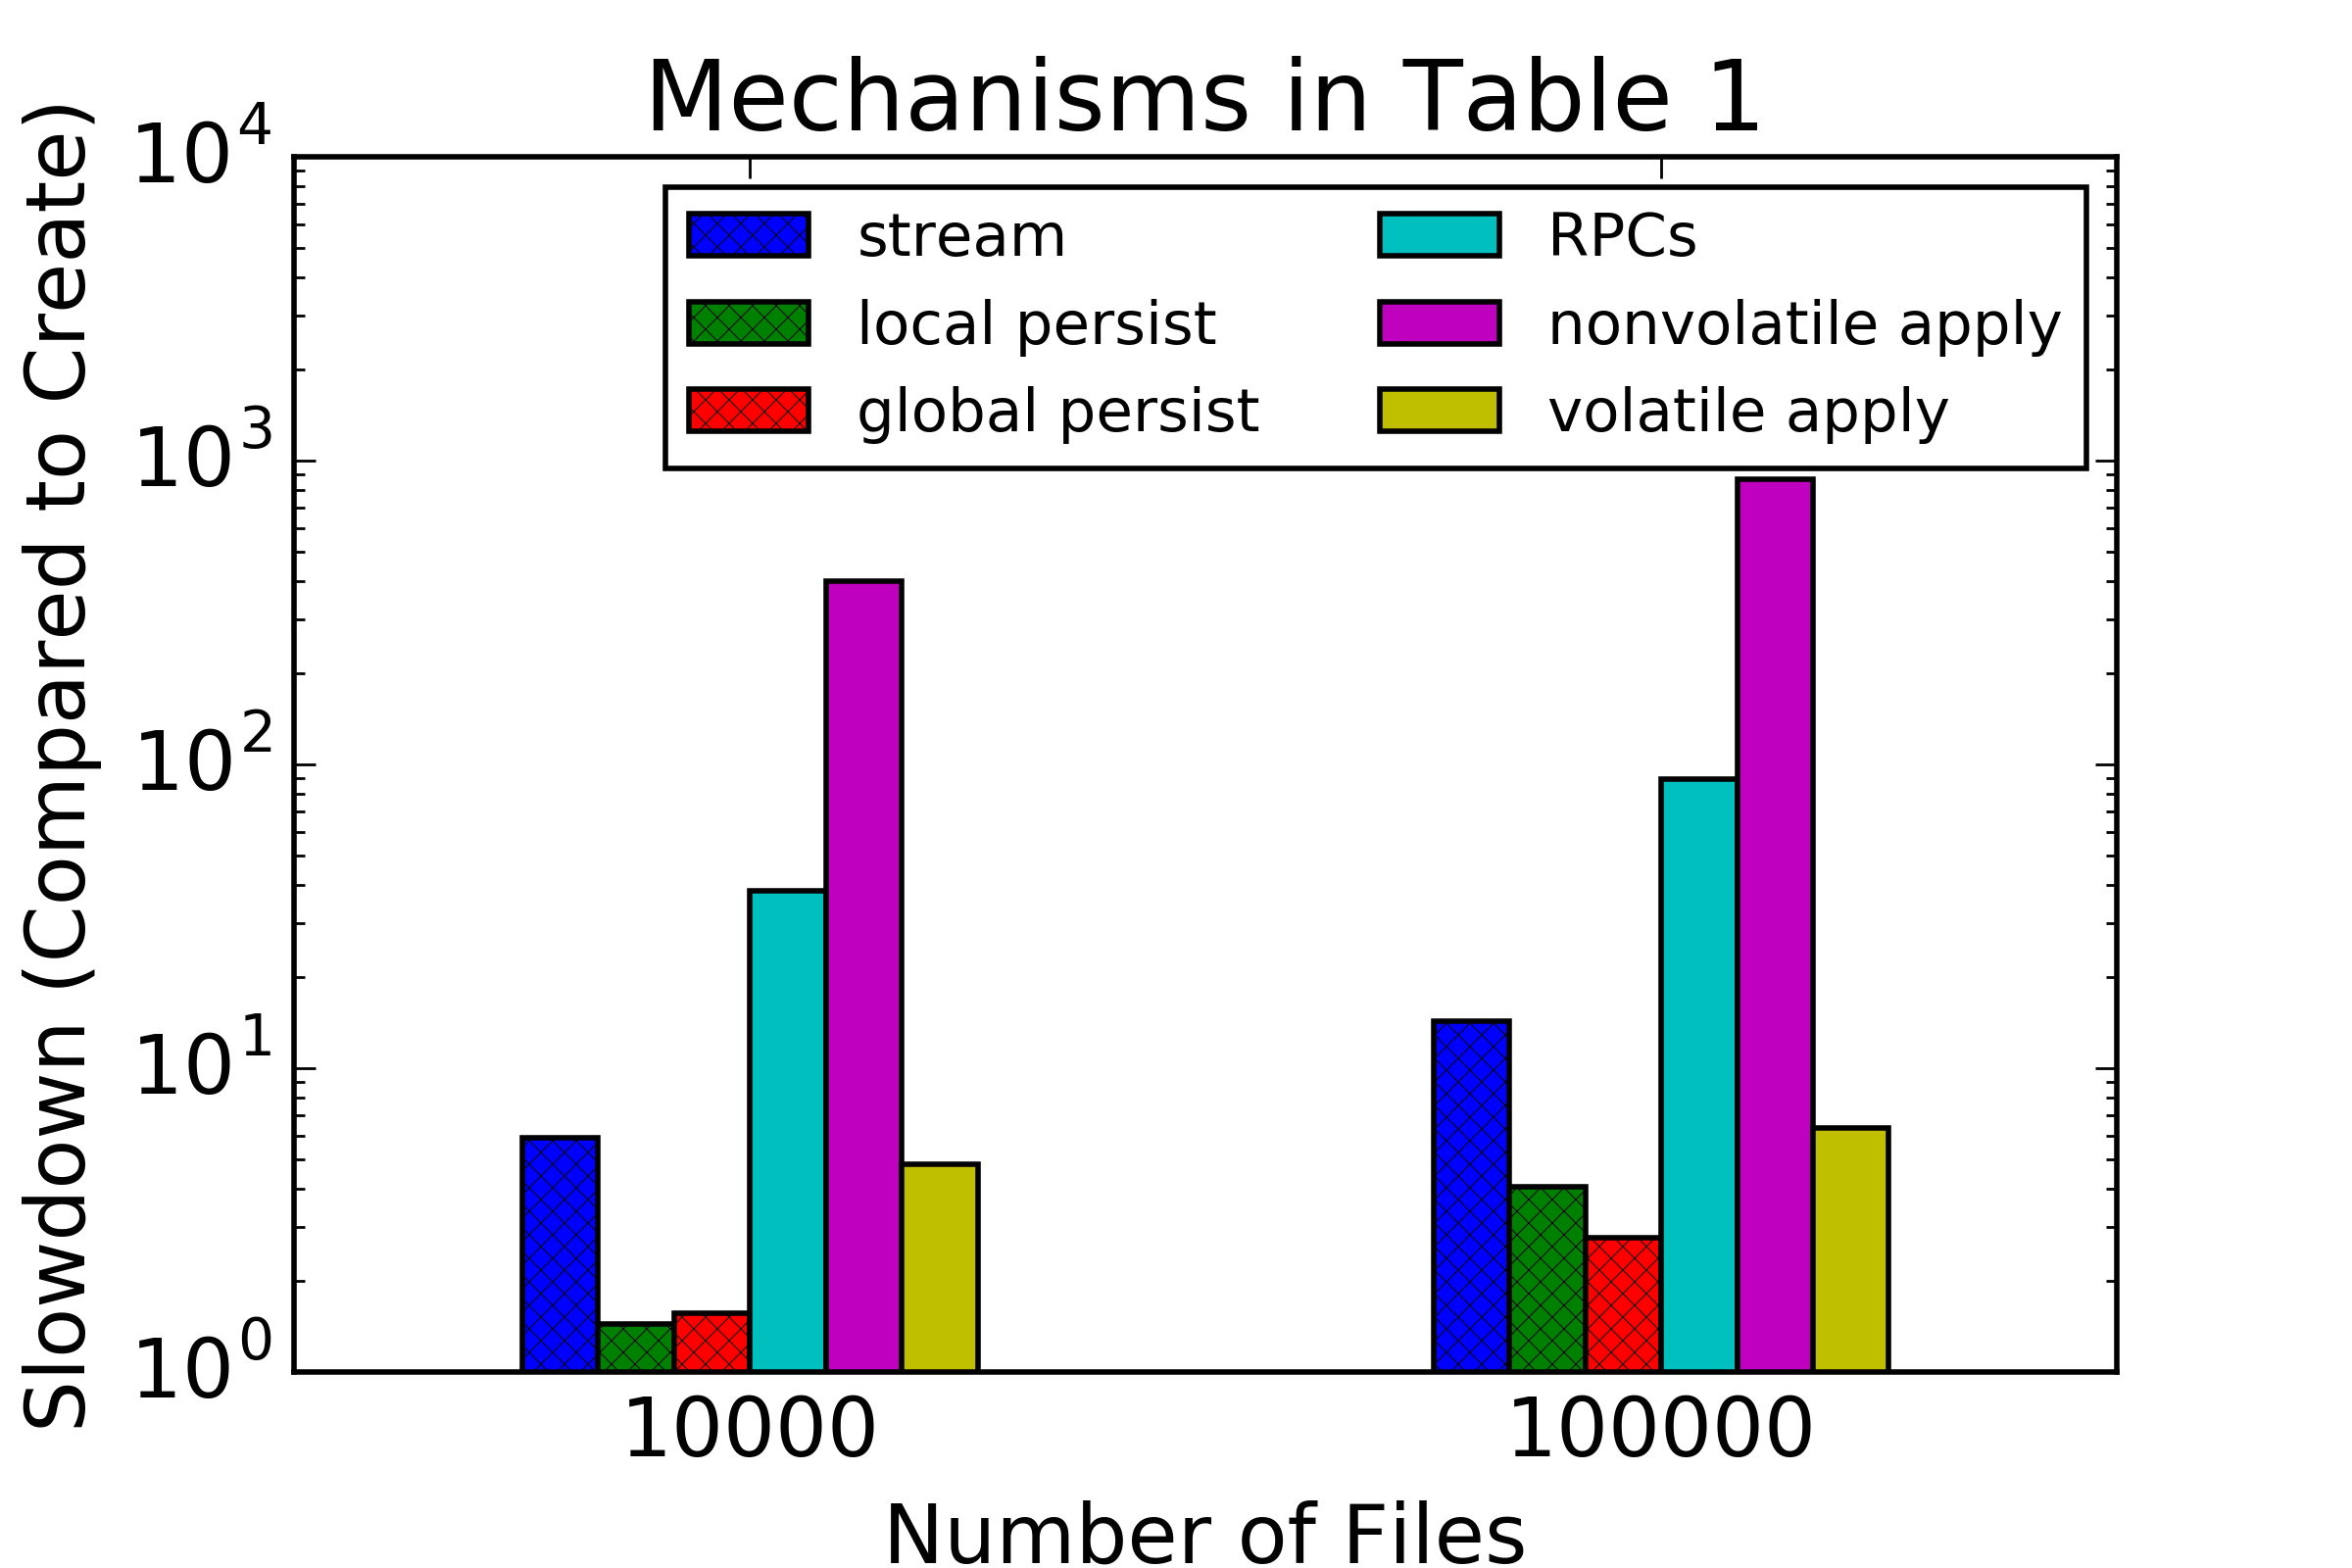
\includegraphics[width=1.0\linewidth]{graphs/slowdown-mechanisms.png}
\caption{
[\href{https://...}{source}]
The performance of the CudeleFS mechanisms normalized to the runtime of the
``Append Client Journal" mechanism (the runtime of writing \(n\) file creates
to the client's in-memory journal).  \label{fig:slowdown-mechanisms}}
\end{figure}

\begin{figure}[tb]
\centering
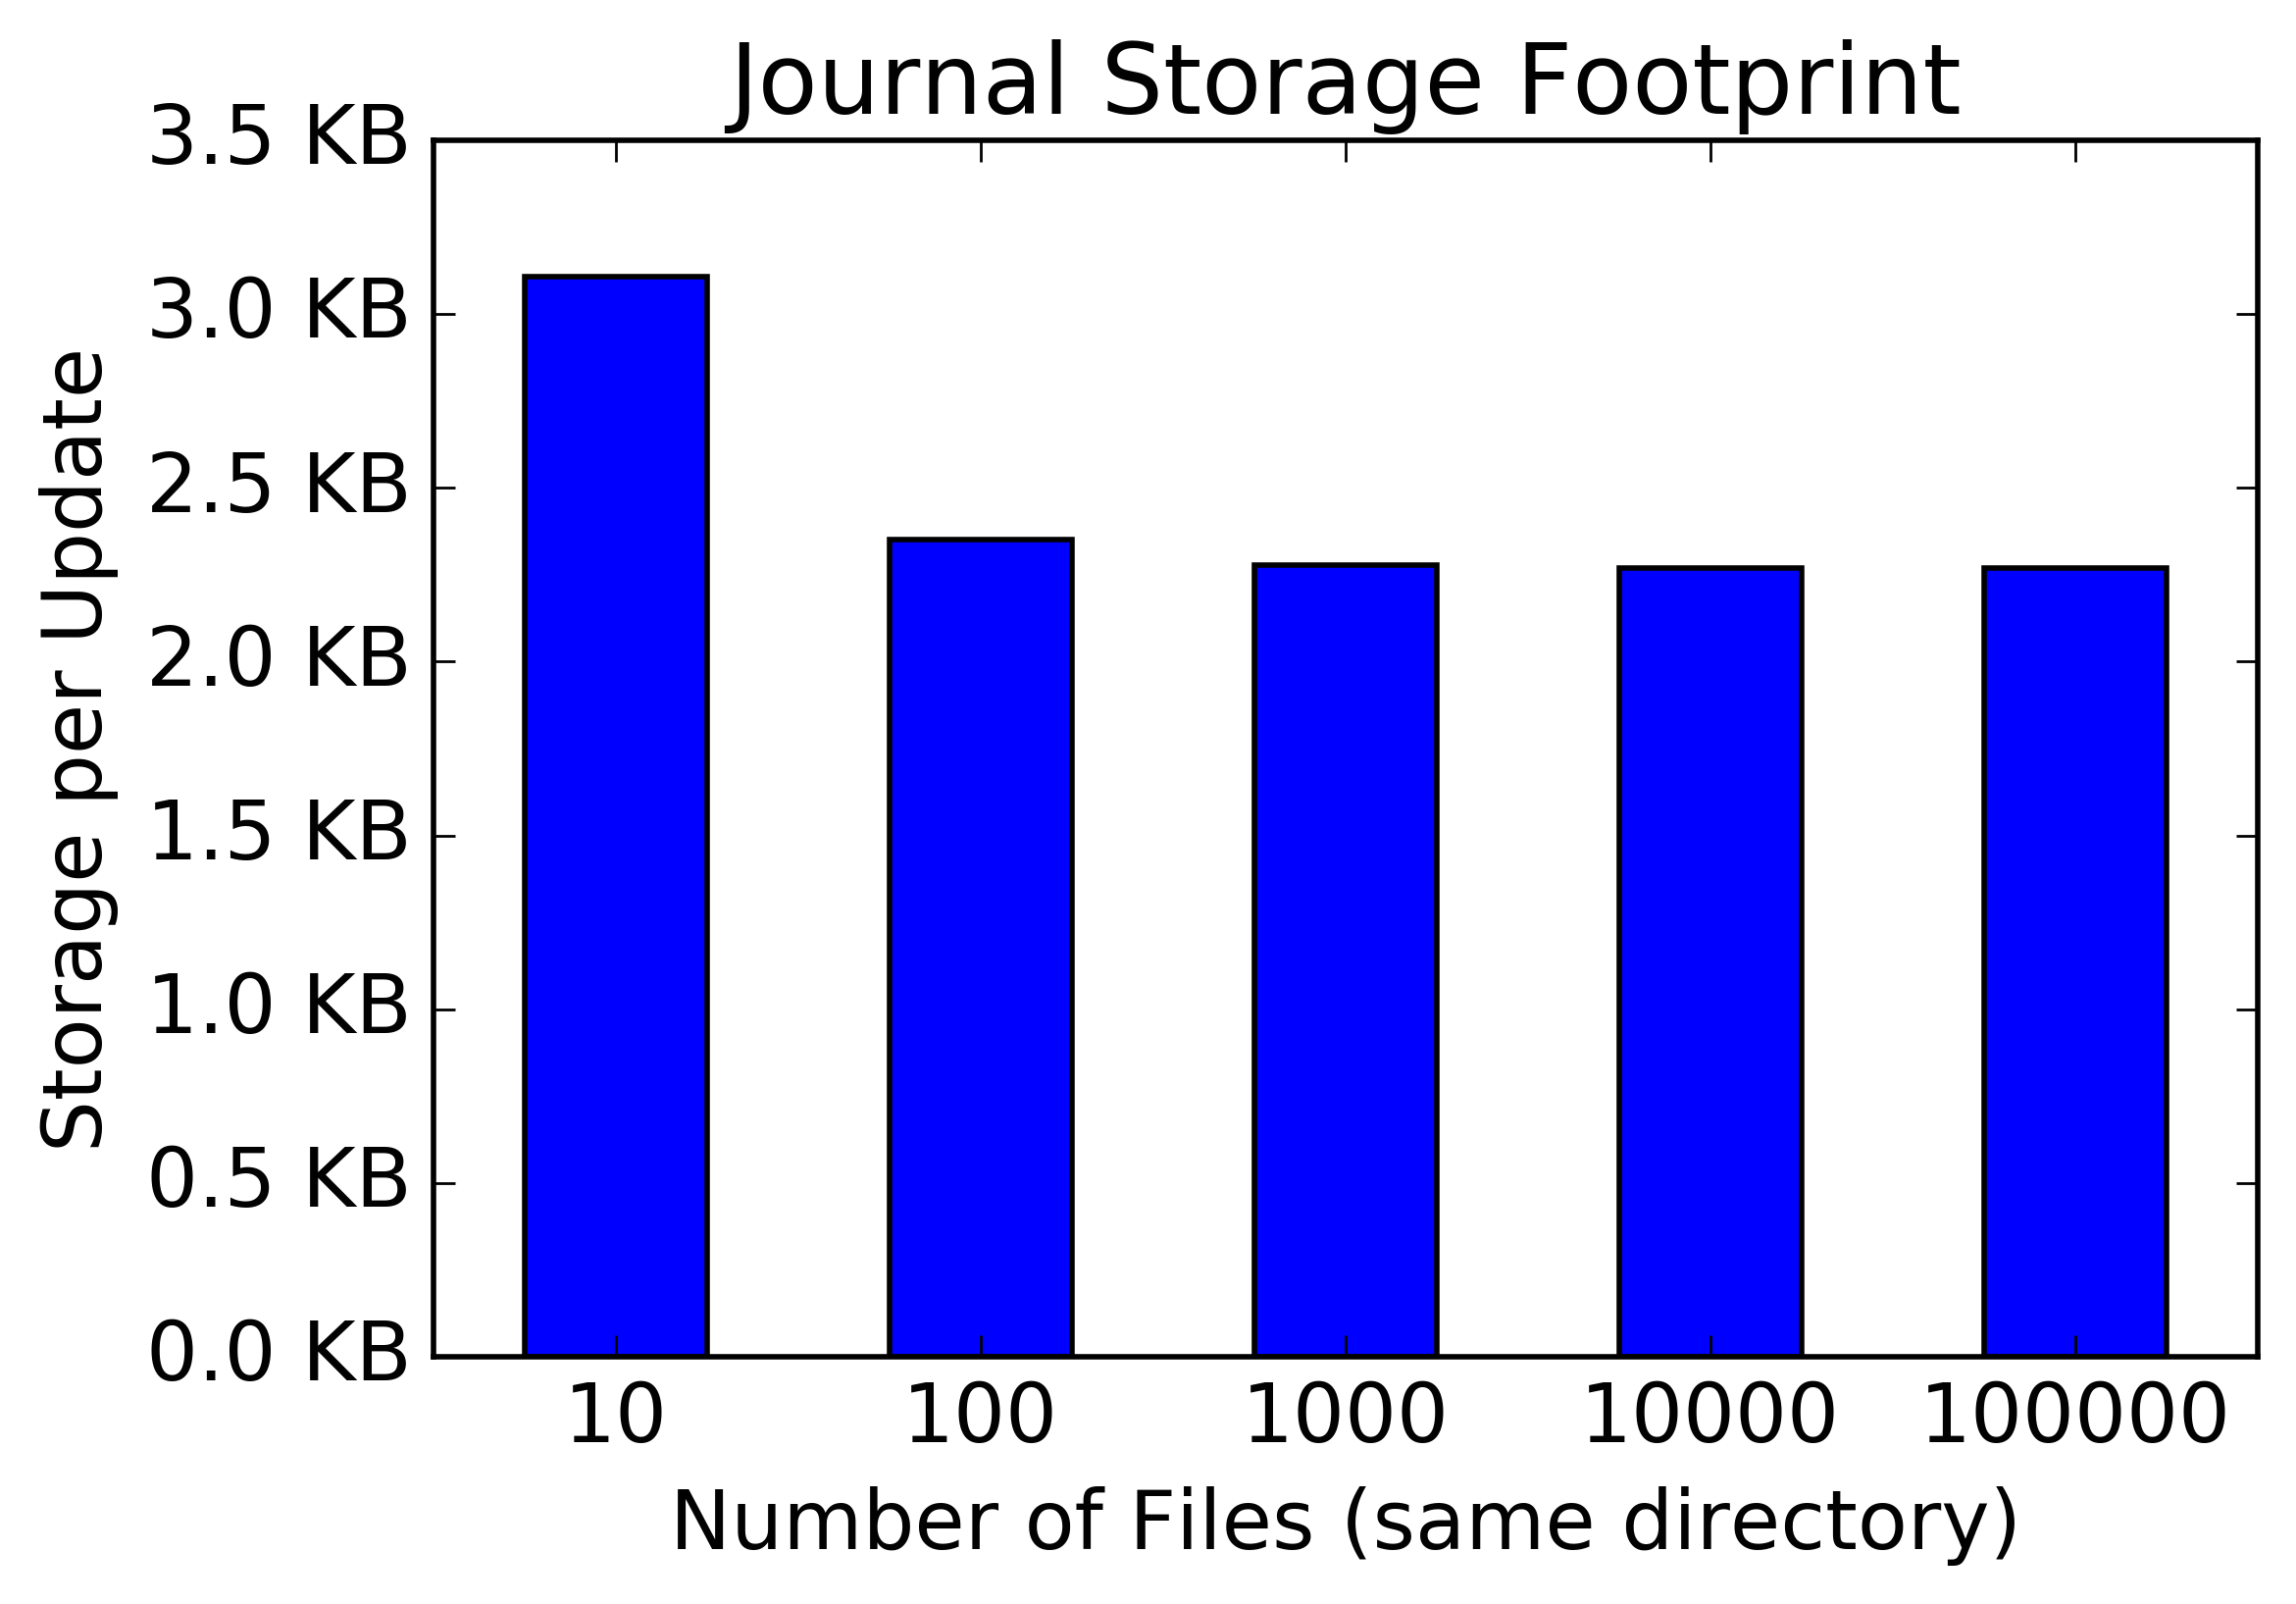
\includegraphics[width=1.0\linewidth]{graphs/behavior-journal-size.png}
\caption{
[\href{https://...}{source}]
In-memory client journal scales with the number of
updates.\label{fig:behavior-journal-size}}
\end{figure}

Figure~\ref{fig:slowdown-mechanisms} shows the runtime of the CudeleFS
mechanisms, normalized to the time it takes to write \(n\) file create updates
to the client's in-memory journal ({\it i.e.} the ``Append Client Journal"
mechanism). Bars above \(10^0\) are slower than the ``Append Client Journal"
mechanism.  ``Stream" is an approximation of the
overhead and is calculated by subtracting the runtime of the job with the
journal turned off from the runtime with the journal turned on.  The largest
workload we tested is 100K file creates in the same directory.  This is the
maximum recommended size of a directory in CephFS; preliminary experiments with
larger directory sizes show memory problems.

\subsubsection{Poorly Scaling Data Structures} Despite doing the same amount of
work, mechanisms that rely on poorly scaling data structures have large
slowdowns for the larger number of creates. For example, ``RPCs" which relies
on the internal CephFS directory structures, goes from a \(40\times\) slowdown
for 10K files to a \(90\times\) slowdown for 100K files. It is a well-known
problem that directory data structures do not scale when creating files in the
same directory~\cite{ren:sc2014-indexfs} and any mechanism that uses these data
structures will experience similar slowdowns. Other mechanisms that write
events to a journal ({\it e.g.} the persists, ``Volatile Apply") experience a
much less drastic slowdown because the journal data structure does not need to
be scanned for every operation. Events are written to the end of the journal without
even checking the validity ({e.g.}, if the file already exists for a create),
which is another form of relaxed consistency because the file system assumes the
application has resolved conflicting updates in a different way.

% RPCs vs. apply: calls to metadata server vs. RADOS
\subsubsection{Overhead of RPCs} ``RPCs" is \(66\times\) slower than ``Volatile
Apply" because sending individual metadata updates over the network is costly.
While ``RPCs" sends a request for every file create, ``Nonvolatile Apply"
writes all the updates to the in-memory journal and applies them to the
in-memory data structures in the metadata server. While communicating the
decoupled namespace directly to the metadata server is faster, communicating
through the object store (``Nonvolatile Apply") is \(10\times\) slower.

% TODO: why is apply so slow.  
% apply: no CephFS changes, pulls/pushes same RADOS obj.
% v_apply vs. apply/persist: communicating through RADOS
\subsubsection{Overhead of ``Nonvolatile Apply"} The cost of ``Nonvolatile
apply" is much larger than all the other mechanisms.  That mechanism was not
implemented as part of CudeleFS -- it was a debugging and recovery tool packaged
with CephFS. It works by iterating over the updates in the journal and pulling
all objects that {\it may} be affected by the update.  This means that two
objects are repeatedly pulled, updated, and pushed: the object that houses the
experiment directory and the object that contains the root directory ({\it
i.e.} \texttt{/}).  The cost of communicating through the object store is shown
by comparing the runtime of ``Volatile apply" + ``Global persist" to
``Nonvolatile Apply". These two operations end up with the same final metadata
state but using ``Nonvolatile Apply" is clearly inferior.

% persist vs. save: one disk vs. many
\subsubsection{Parallelism of the Object Store} Comparing ``Local" and ``Global
persist" demonstrates the bandwidth advantages of storing the journal in a
distributed object store. For 100K file creates, the ``Global Persist"
performance is \(1.5\times\) faster because the object store is leveraging the
collective bandwidth of the disks in the cluster. This benefit comes from the
object store itself but should be acknowledged when making decisions for the
application; the size of the object store can help mitigate the overheads of
globally persisting metadata updates.

\subsubsection{Journal Size} Figure~\ref{fig:behavior-journal-size} shows the
amount of storage per journal update (\(y\) axis) for the range of file creates
we tested (\(x\) axis). The increase in file size is linear with the number of
metadata creates and suggests that updates for a million files would be
\(2.5\text{KB}*1\text{ million files} = 2.38\text{GB}\). Transfer times for
payloads of this size on an HPC network are reasonable.\\

\noindent\textbf{Takeaway}: the CudeleFS mechanisms have overheads and costs
that can differ {\it by orders of magnitude}. CudeleFS gives users the ability
to compose these mechanisms based on their application's correctness
requirements and performance goals.

\subsection{Weak vs. Strong Consistency}
\begin{figure}[tb]
\centering
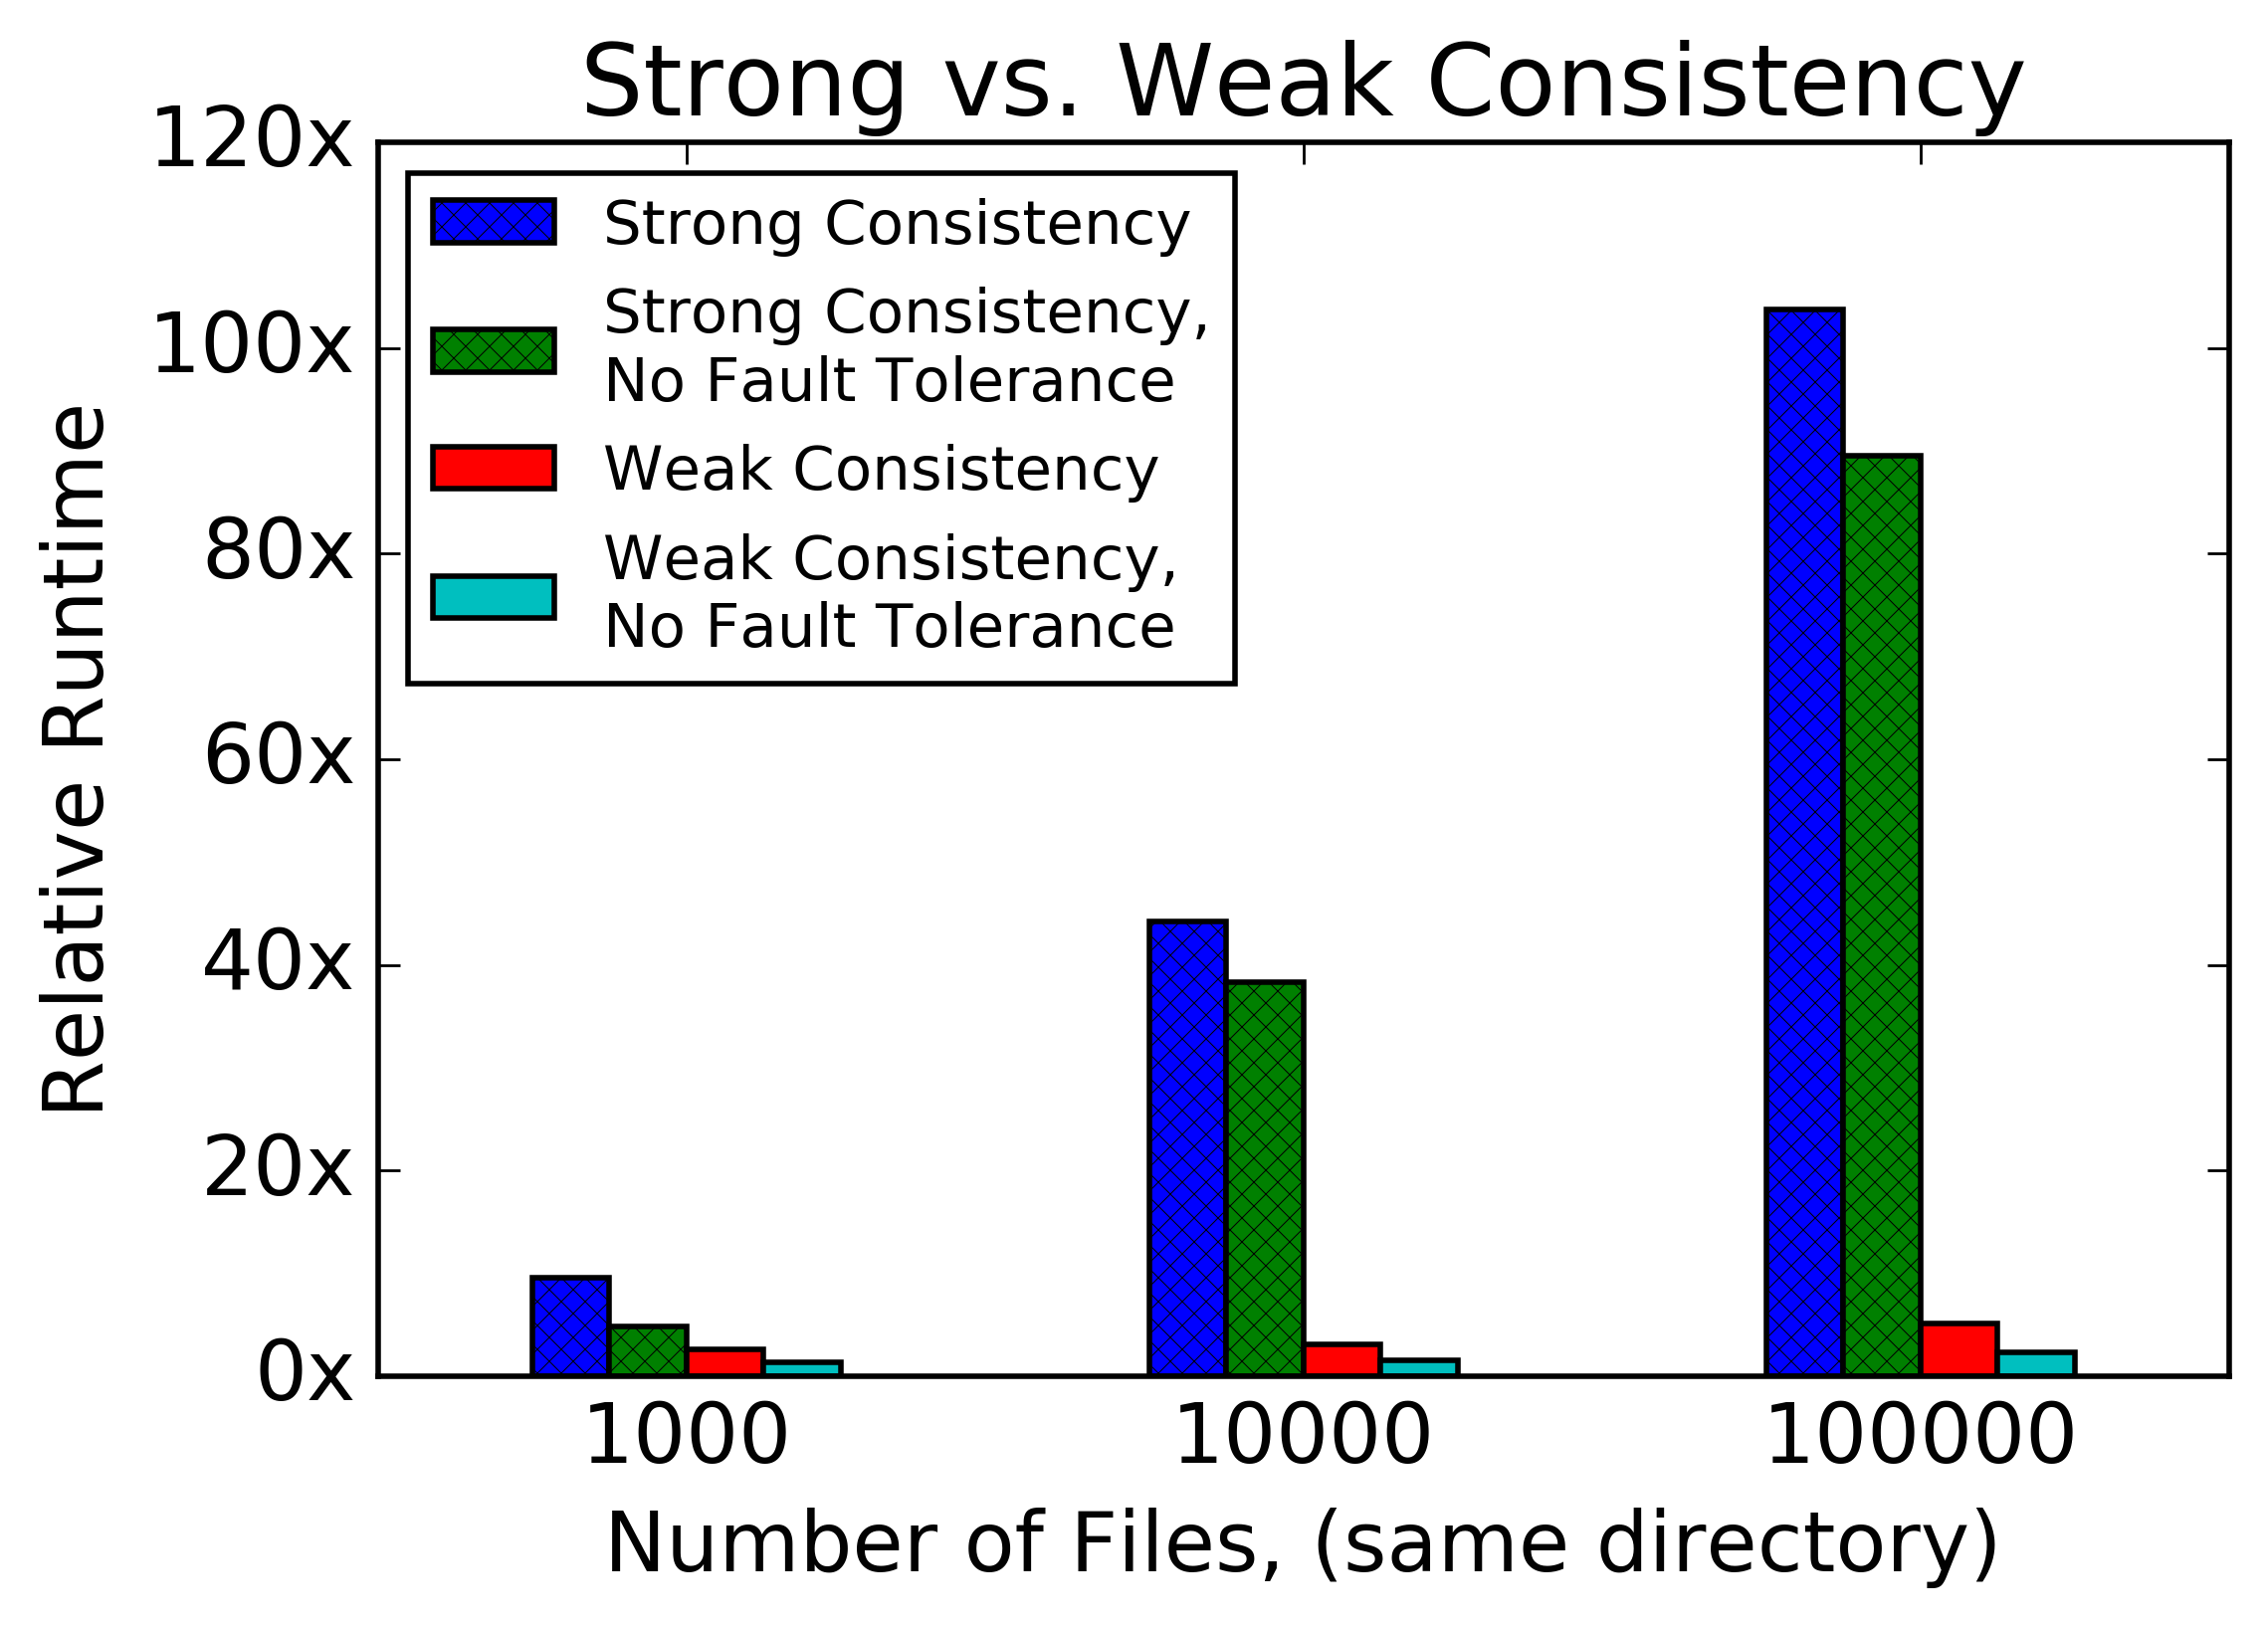
\includegraphics[width=1.0\linewidth]{graphs/slowdown-strong-v-weak.png}
\caption{
[\href{https://...}{source}]
The RPC per metadata update of ``Strong Consistency" has a large
overhead compared to the decoupled namespace strategy of ``Weak
Consistency".\label{fig:slowdown-strong-weak}}
\end{figure}

Figure~\ref{fig:slowdown-strong-weak} shows the runtime of systems employing
weak and strong consistency, normalized to the runtime of the ``Append Client Journal"
mechanism (again, just creating files in the client's in-memory journal).  We
use the following compositions from the mechanisms in
Table~\ref{table:spectrum}:  Strong Consistency = ``RPCs" + ``Stream"; Strong
Consistency, No Fault Tolerance = ``RPCs"; Weak Consistency = ``Append Client Journal" +
``Local Persist"; and Weak Consistency, No Fault Tolerance = ``Append Client Journal" +
``Local Persist" + ``Volatile Apply".

% Final file system metadata states are equivalent No guarantees while
% transitioning mechanisms
We compare these semantics because the final metadata states are equivalent.
CudeleFS makes no guarantees during execution of the mechanisms or when
transitioning semantics -- the semantics are guaranteed {\it once the mechanism
completes}. So if servers fail during a mechanism, metadata or data may be
lost.

% DeltaFS vs. BatchFS vs. POSIX: decoupled is faster
% (5-7x) vs. (90-104x) slower
% Does not scale?
% Strong Consistency > 10X slower than Weak Consistency 
\subsubsection{Speedups of Decoupled Namespaces} Weak consistency uses the
decoupled namespace strategy and shows up to a \(20\times\) speedup over the
traditional namespaces that use RPCs. Compared to the baseline the slowdown is
\(5-7\times\) for Strong Consistency, which emulates BatchFS and
\(90-104\times\) for Weak Consistency, which emulates DeltaFS.

% POSIX (no stream) vs. POSIX: cost of durability < consistency
\subsubsection{Durability \(<<\) Consistency} The \(1.15\times\) overhead of
Strong Consistency compared to Strong Consistency, No Fault Tolerance for
100K files is negligible. It suggests that the overhead of consistency is much
larger than the overhead of durability. This conclusion should be stronger as
we scale the number of files because the cost of streaming the journal into the
object store is constant. We omit the same analysis for Weak Consistency
because the runtimes are so short that the normalized slowdowns are misleading.

% Weak Consistency benefit not due to metadata format
\subsubsection{Metadata Formats} Because the metadata formats are the same for
all schemes we argue that the performance gain for decoupled namespaces comes
from relaxing the consistency guarantees and not from the metadata formats, as
was argued in previous work outlining the benefit of
SSTables~\cite{ren:atc2013-tablefs, ren:sc2014-indexfs}.\\

\noindent\textbf{Takeaway}: CudeleFS shows the true benefit of eventual
consistency, where we see over a \(100\times\) slowdown for achieving strong
consistency, in the worst case.

%\section{notes}
%Linking clients into our custom libcephfs
%
%Use namespace's recursive data structure to put policies on subtrees
%- consistency: weak vs. strong, global vs. local
%  - e.g., BatchFS/DeltaFS: weak, local
%  - e.g., POSIX: strong, global
%  - e.g., PLFS: no consistency
%- durability: global vs. local
%  - e.g., CephFS: global
%  - e.g., BatchFS/DeltaFS: local
%
%Experimental Setup
%- Ceph: 9 OSDs, 1 metadata server, 2 kernel client
%- Workload limitations: blah
%
%Workload: creates
%
%Baseline: 200K creates in the same directory
%- throughput: degrades at 950s
%- CPU utilization: more at 950s
%- inode cache: eviction dominate
%- inodes +- to cache: eviction dominate
%- per-disk throughput: RADOS not bottleneck
%
%Experiment 1: Interference
%
%\subsection{Baseline}
%Experiment 0: creates in the same directory
%- setup: why we use caching, we use the kernel client, how we circumvent max fragment size
%
%Experiment 0: creates with a stat
%- Hypothesis: metadata read pauses creates and requires a snapshot in time
%  - what is more of an overhead: pausing creates and getting a consistent view OR sucking up resources as it reads from RADOS?
%- can we delay snapshot?
%
%Experiment 1: creates with a readdir
%- Hypothesis: shows the cost of synchronization because on a write, the first client drops his caps
%- client0: create 100k, client1: stat at 2 mins
%
%Experiment 2: scale the number of files
%- See if the open/close spike occurs 
%- Try to see why open/close spike is allowed to happen
%- Try to disable all caching -- metadata writes don't ever re-use the inode -- we never ask for it again!
%- client0: create 100k, client1: touch at 2 mins
%
%Experiment 3: see how fast the cache satisfies a read
%- client0: create 100k, stat inodes
%- client0: create 100k, client1: stat inodes
%
%lient 0: creates, client 1 create(s)

\subsection{Benefits of Isolated Subtree Policies}

\begin{figure}[tb]
\centering
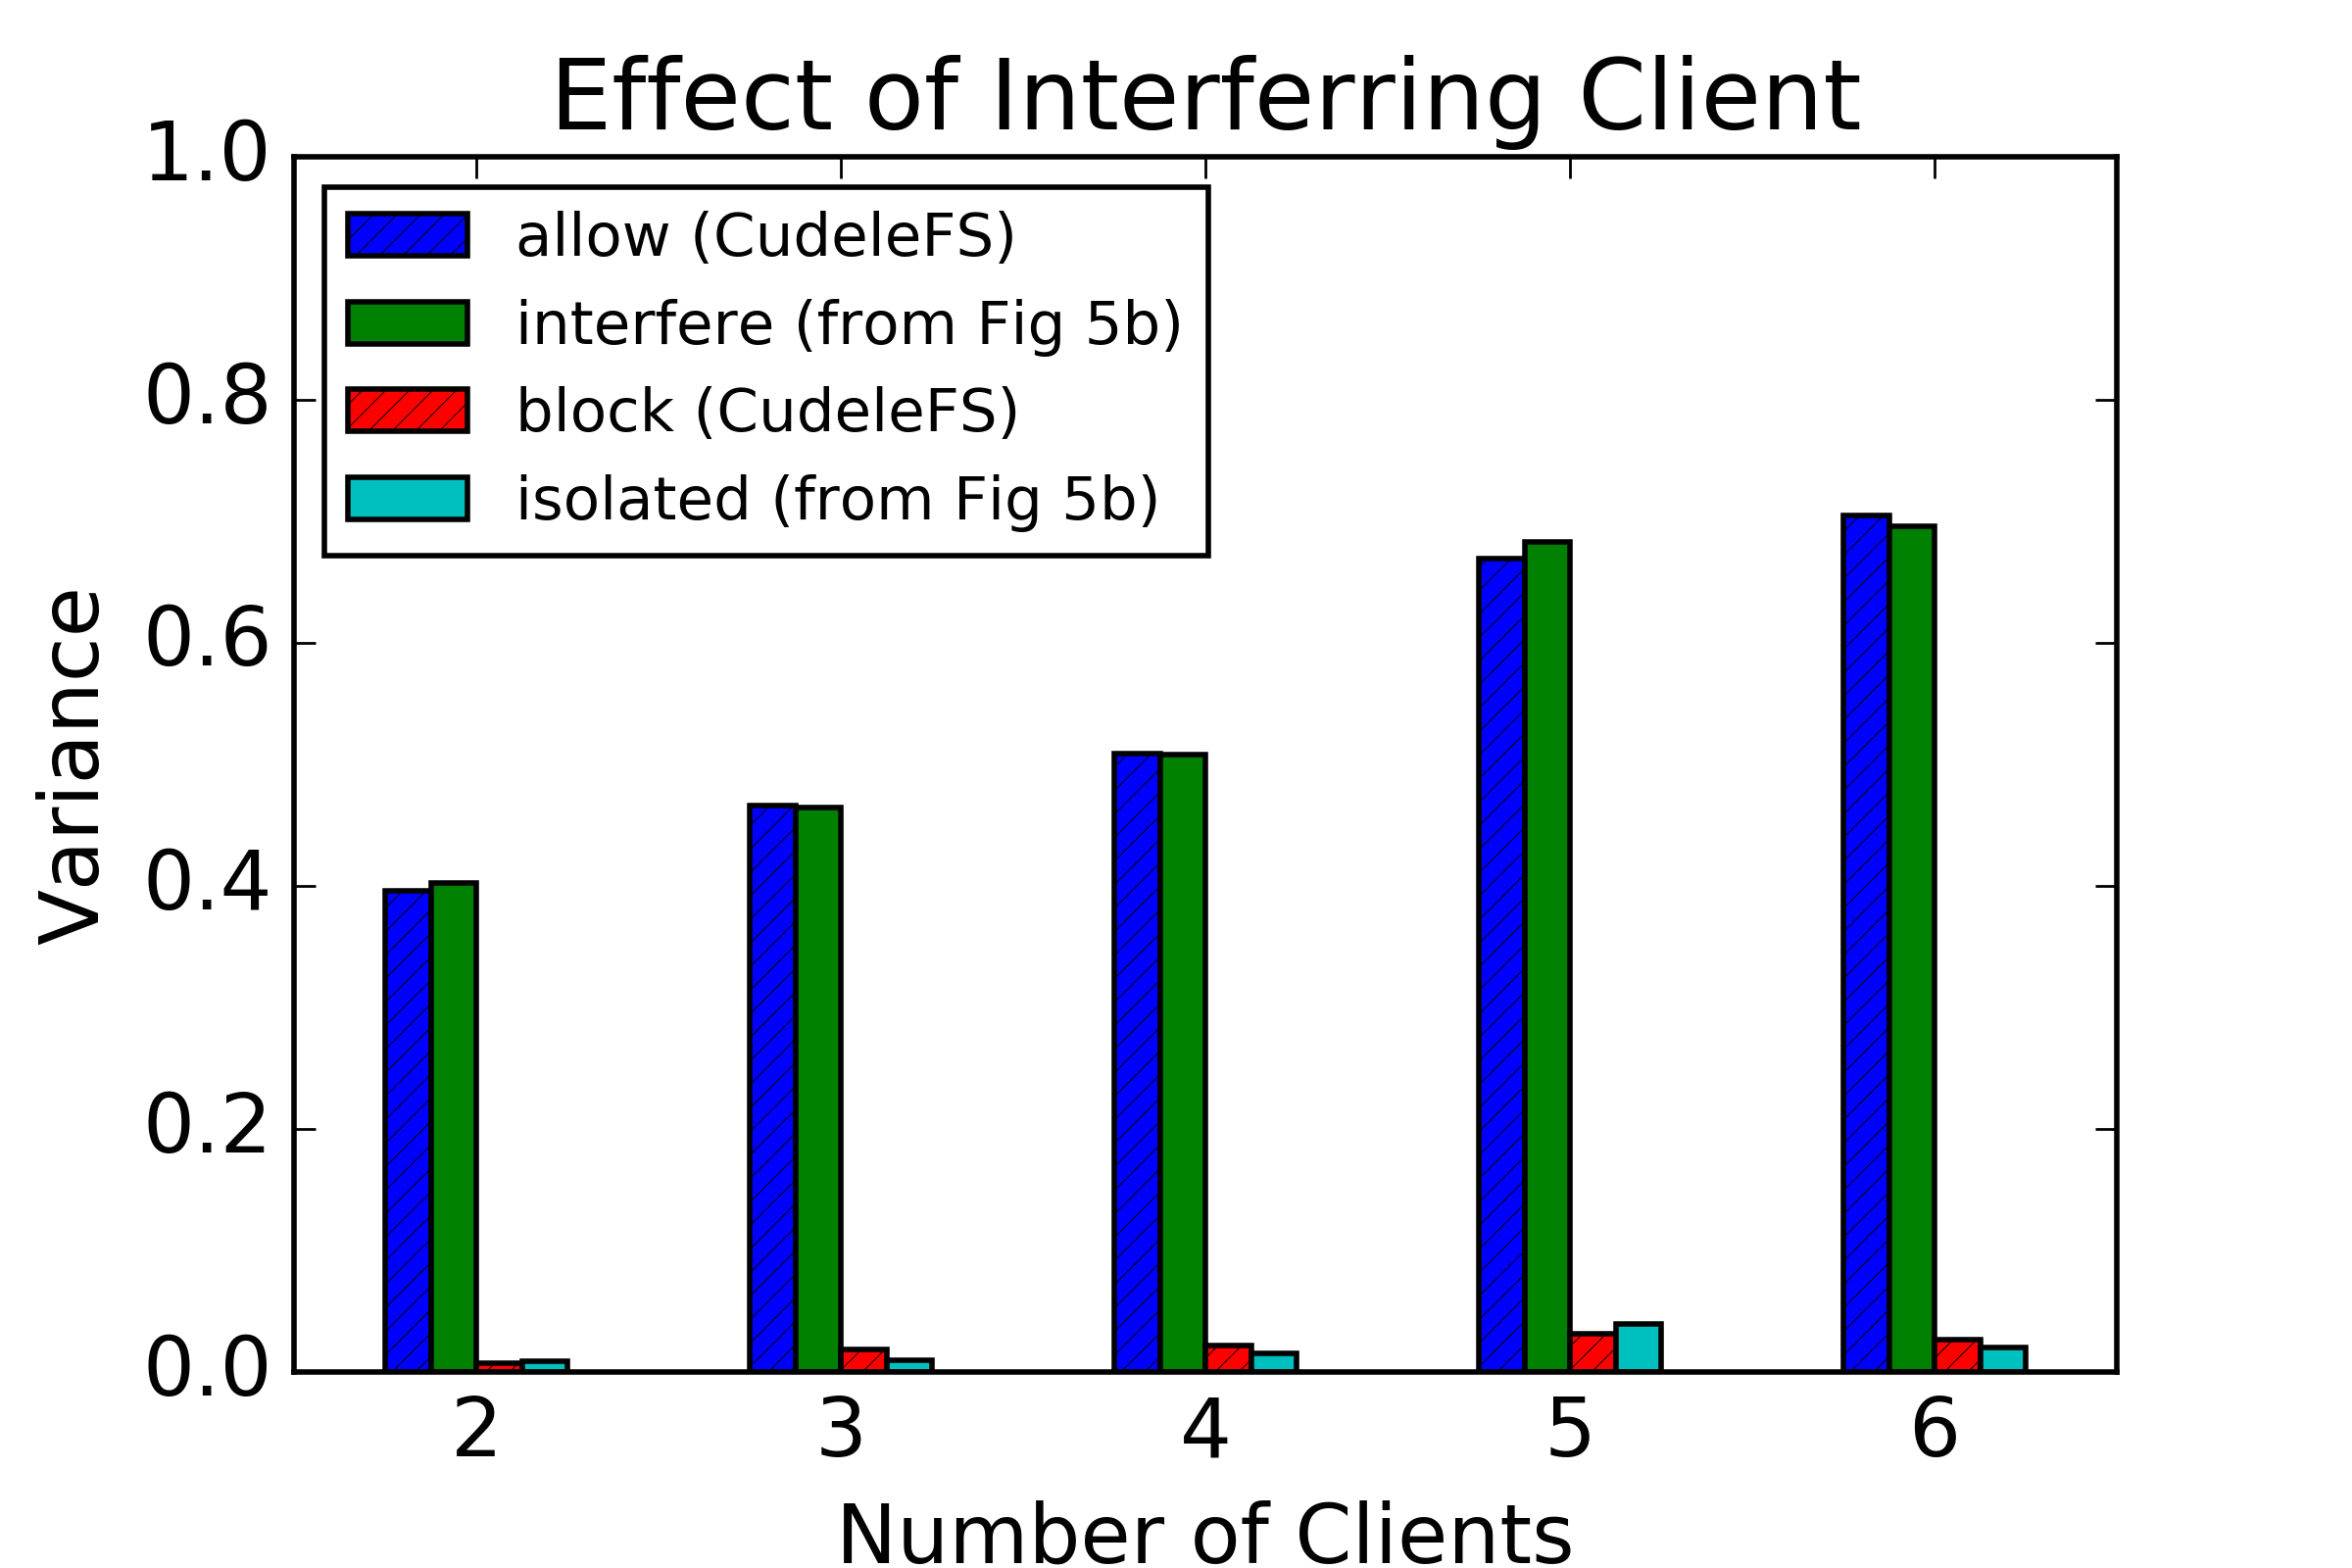
\includegraphics[width=1.0\linewidth]{graphs/slowdown-allow-block.png}
\caption{
[\href{https://...}{source}]
Using the ``allow" and ``block" API, users can isolate directories from
interfering clients. Performance with blocking turned is the same as
``isolated" from Figure~\ref{fig:overhead-b}.
\label{fig:slowdown-allow-block}}
\end{figure}

% setup: 2cs sep dirs, 2cs DN, 1c malicious write
Next we show how CudeleFS can be programmed to block interfering clients. We
use the same problematic workload from Figure~\ref{fig:overhead-b}, where
clients write to their own private directories and another client interferes with a stream of creates at
30 seconds.  We also have another client write to a decoupled namespace and
merge its updates at 90 seconds.  We equip each client directory with the
configuration:

\begin{listing}[tb]
\begin{minted}[xleftmargin=21pt,
               tabsize=4]{js}
{     
    "allocated_inodes": "100000"
    "interfere_policy": "block"
    "consistency": "RPCs"
    "durability": "stream"
}
\end{minted}
\end{listing}

Each directory functions with ``RPCs"
and ``Stream" enabled -- which is the default implementation of CephFS. The only
difference is that we enable blocking on each subtree so while the tree behaves
like CephFS, all interfering operations will be returned with \texttt{-EBUSY}.
Note that IndexFS does a similar operation with leases except clients block.

% results
To show the benefits of this isolations, our results in
Figure~\ref{fig:slowdown-allow-block} are plotted alongside the variance bars from
Figure~\ref{fig:interfere-b}. Because ``allow"/``interfere and
``block"/``isolated" have the same variability we draw the following three
conclusions: (1) clients that use the API to block interfering clients  get
the same performance as isolated clients, (2) there is a negligible effect on
performance for the extra work the metadata server does to return
\texttt{-EBUSY}, and (3) merging updates from the decoupled client has a
negligible effect on performance.\\

\noindent\textbf{Takeaway}: the API lets users isolate directories when
applications need better and more reliable performance. This is a way of
controlling consistency.

\subsection{Scaling Concurrent Merges}

Figure~\ref{boner} scales the number of merges and shows linear performance.
The performance is linear for two reasons: (1) the merges are serialized and
(2) applying the updates to the in-memory metadata store does not touch data
structures that scale poorly. CudeleFS serializes merge requests 

\subsection{Partial Directory Listings}
